\documentclass[xcolor=x11names,compress]{beamer}

%% General document %%%%%%%%%%%%%%%%%%%%%%%%%%%%%%%%%%
\usepackage{graphicx}
\graphicspath{{graphics/}}
\usepackage{tikz}
\usepackage{color,colortbl}
\usepackage{framed}
\usepackage{textcomp, setspace} %Needed for customization of ``listings''
% package
\usepackage[procnames]{listings} % to display code; don't forget [fragile]
% option after \begin{frame}
\input{inputs/rgb}
\definecolor{shadecolor}{rgb}{1,.9,.3}

\usepackage [autostyle]{csquotes}
\MakeOuterQuote{"}

\lstset{
    backgroundcolor=\color{shadecolor},
    tabsize=4,
    rulecolor=,
    language=python,
        basicstyle=\ttfamily\setstretch{1},
        upquote=true,
        aboveskip={1.5\baselineskip},
        columns=fixed,
        showstringspaces=false,
        extendedchars=true,
        breaklines=true,
        prebreak = \raisebox{0ex}[0ex][0ex]{\ensuremath{\hookleftarrow}},
        frame=single,
        showtabs=false,
        showspaces=false,
        showstringspaces=false,
        identifierstyle=\ttfamily,
        keywordstyle=\color[rgb]{0,0,1},
        commentstyle=\color[rgb]{0.133,0.545,0.133},
        stringstyle=\color[rgb]{0.627,0.126,0.941},
        numbers=left, 
        numberstyle=\tiny, 
        stepnumber=2, 
        numbersep=5pt
}

%%%%%%%%%%%%%%%%%%%%%%%%%%%%%%%%%%%%%%%%%%%%%%%%%%%%%%

%% Beamer Layout %%%%%%%%%%%%%%%%%%%%%%%%%%%%%%%%%%
\usetheme{Madrid}
\usecolortheme{seahorse}
\useoutertheme[subsection=false,shadow]{miniframes}
\useinnertheme{default}
% \usefonttheme{serif}
\usepackage{palatino}

\setbeamerfont{title like}{shape=\scshape}
\setbeamerfont{frametitle}{shape=\scshape, series = \bfseries}
\setbeamertemplate{frametitle}[default][center]
\setbeamertemplate{headline}{} %suppress headline (navigation pane)

\setbeamertemplate{footline}
{
  \leavevmode%
  \hbox{%
%   \begin{beamercolorbox}[wd=.4\paperwidth,ht=2.25ex,dp=1ex,center]{author in 
% head/foot}%
%     \usebeamerfont{author in head/foot}\insertshortauthor
%   \end{beamercolorbox}%
  \begin{beamercolorbox}[wd=.93\paperwidth,ht=2.25ex,dp=1ex,left]{title in 
head/foot}%
    \usebeamerfont{title in head/foot}\insertshorttitle\hspace*{3em}
  \end{beamercolorbox}}%
  \begin{beamercolorbox}[wd=.07\paperwidth,ht=2.25ex,dp=1ex,center]{}
     \insertframenumber{} / \inserttotalframenumber\hspace*{1ex}
%       \insertframenumber{}
  \end{beamercolorbox}

}
% \setbeamercolor*{lower separation line head}{bg=DeepSkyBlue4} 
% \setbeamercolor*{normal text}{fg=black,bg=white} 
% \setbeamercolor*{alerted text}{fg=red} 
% \setbeamercolor*{example text}{fg=black} 
% \setbeamercolor*{structure}{fg=black}
%  
% \setbeamercolor*{palette tertiary}{fg=black,bg=black!10} 
% \setbeamercolor*{palette quaternary}{fg=black,bg=black!10} 

\renewcommand{\(}{\begin{columns}}
\renewcommand{\)}{\end{columns}}
\newcommand{\<}[1]{\begin{column}{#1}}
\renewcommand{\>}{\end{column}}

\def\signed #1{{\leavevmode\unskip\nobreak\hfil\penalty50\hskip2em
  \hbox{}\nobreak\hfil(#1)%
  \parfillskip=0pt \finalhyphendemerits=0 \endgraf}}

\newsavebox\mybox
\newenvironment{aquote}[1]
  {\savebox\mybox{#1}\begin{quote}}
  {\signed{\usebox\mybox}\end{quote}}

% \title{CMEE Masters Week 6: Python week II}
\title{VectorBiTE Training: Model fitting}
\author{Samraat Pawar}
  
%%%%%%%%%%%%%%%%%%%%%%%%%%%%%%%%%%%%%%%%%%%%%%%%%%%%

\begin{document}

%%%%%%%%%%%%%%%%%%%%%%%%%%%%%%%%%%%%%%%%%%%%%%%%%%%%%%
\begin{frame}[plain]

% \title{Fitting Models to Data in Ecology and Evolution}
\title{Fitting Models to Data in Vector-Borne Disease Systems}
% \vspace{12pt}
% \subtitle{CMEE Masters}
\author{
    Samraat Pawar\\
    \vspace{20pt}
  \centering
%   \includegraphics[height = .3in]{Imperial_Color1.pdf}\\
  
\includegraphics[height = .5in]{../../notebooks/graphics/VB_logo.jpg}
}
 
\titlepage
\end{frame}

%%%%%%%%%%%%%%%%%%%%%%%%%%%%%%%%%%%%%%%%%%%%%%%%%%%%%%
\begin{frame}{Mechanisms in vector-borne disease dynamics?}

\begin{center}
	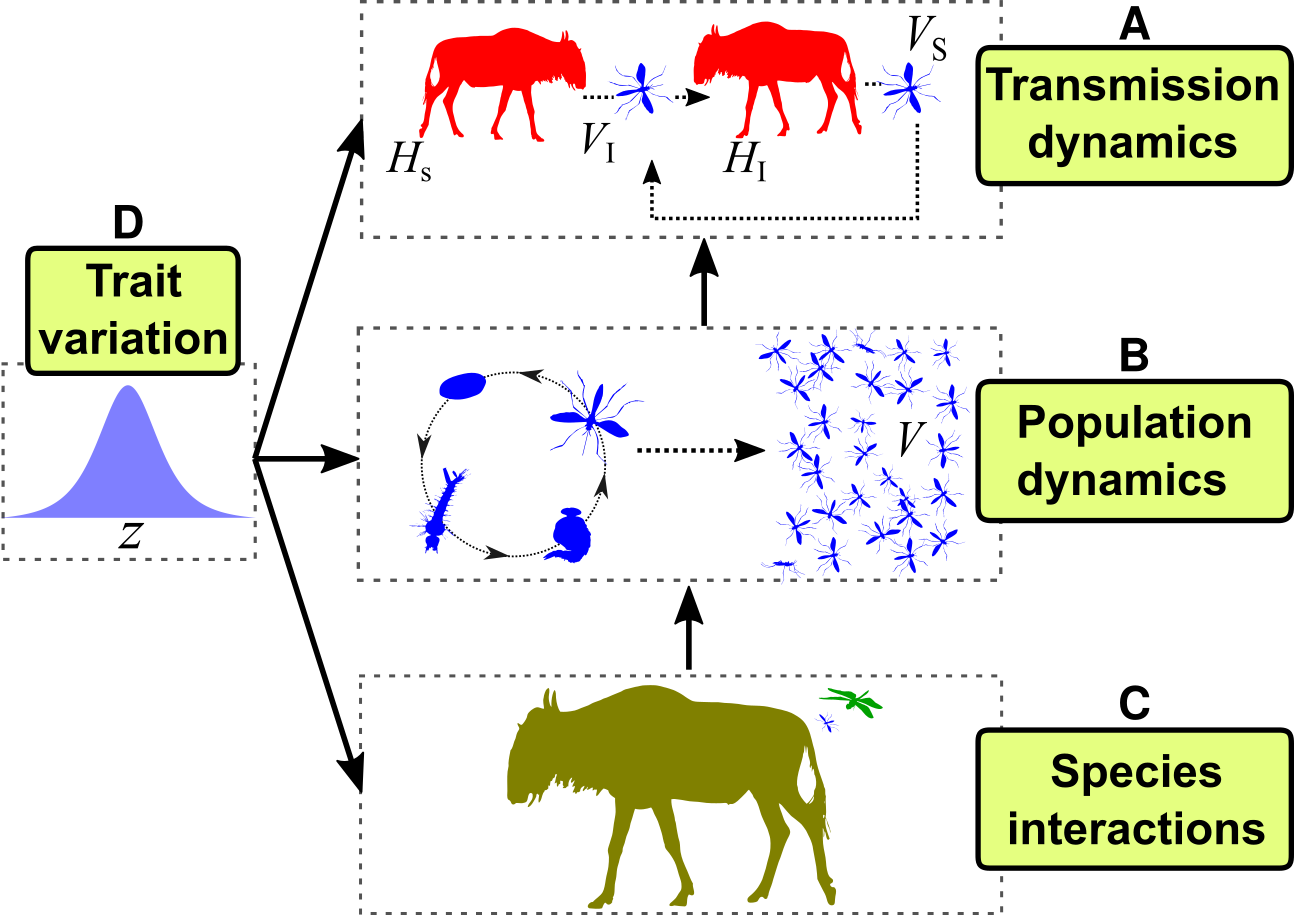
\includegraphics[width=.8\textwidth]{VecTraitOverview.png}	
\end{center}

\end{frame}
	
%%%%%%%%%%%%%%%%%%%%%%%%%%%%%%%%%%%%%%%%%%%%%%%%%%%%%%
\begin{frame}{Mechanistic vs. phenomenological models}

	\begin{itemize}\itemsep4pt
		  \item Mechanistic models aim to explain the PROCESSES underlying 
		  observed patterns
 
		 \item Empirical or phenomenological models show relationships 
		 between observed data (e.g. vector population size or disease incidence as a function of temperature or rainfall), but provide no insights into the processes/mechanisms that inter-link these data.
	  \end{itemize}
 
 \pause
	 
  \begin{center}
	  \includegraphics[width=\textwidth]{Mechanisms.pdf}
  \end{center} 
 
 \end{frame}
 
 %%%%%%%%%%%%%%%%%%%%%%%%%%%%%%%%%%%%%%%%%%%%%%%%%%%%%%
\begin{frame}{Mechanisms in vector-borne disease dynamics?}

\begin{itemize}[<+->] \itemsep12pt
	\item Ecological studies often focus on explaining phenomena 
	using somewhat phenomenological models. 
	
	\item For example, disease invasions, outbreaks and spread: Why cycles? Why traveling waves? 
	
	\item What mechanisms operate? Vector-parasite interaction? Vector-environment interaction? 

\end{itemize}

\end{frame}

%%%%%%%%%%%%%%%%%%%%%%%%%%%%%%%%%%%%%%%%%%%%%%%%%%%%%%
\begin{frame}{What are Mechanisms?}

   \begin{itemize}[<+->] \itemsep4pt{}
			\item Somewhat subjective! 
			\item For example, the Ricker model can be thought of as 
			mechanistic:
			\begin{equation} 
				N_{t+1} = N_t e^{r\left(1-\frac{N_t}{k}\right)} 
			\end{equation} 
				
			\item What is the mechanism? --- Density dependence through scramble competition 
			(Brannstrom \& Sumpter 2005)

			\item If the Ricker model and another model with contest 
			competition were compared with data --- some would call it mechanistic 
			modelling because one is trying to get at the underlying 
			mechanism, scramble or contest competition
			
			\item But is this REALLY mechanistic? What are $r$ and $k$ really?
	
			\item Many (including yours truly!) now argue that we have not 
			progressed far enough because the first level has been ignored!
   \end{itemize}

\end{frame}

%%%%%%%%%%%%%%%%%%%%%%%%%%%%%%%%%%%%%%%%%%%%%%%%%%%%%%
\begin{frame}{An example of a fundamental mechanism: metabolism (Trait)}
      
\begin{columns}[c]
  \column{2.1in}
    \pause
      \includegraphics[width=\textwidth]{graphics/Photobacterium.pdf}
  \pause
  \column{2.7in}
    $B = B_0 \boxed {e^{-\frac{E}{kT}}}f(T,T_{pk},E_D)$\\
    \vspace{10pt}
    \raggedright{$T$ = temperature (K)\\
     $k$ = Boltzmann constant (eV K$^{-1}$)}\\
     $E$ = Activation energy (eV)\\
     $T_{pk}$ = Temperature of peak performance\\
     $E_D$ = Deactivation energy (eV)\\
    {\small (J H van't Hoff 1884, S Arrhenius 1889)}
\end{columns}

\begin{itemize}\setlength{\itemindent}{0em}
  \pause
  \item Surely there is more to thermal responses?
    \begin{itemize}\setlength{\itemindent}{-1em}
     \item Oxygen limitation
     \item Complexity of metabolic network
     \item Hormonal regulation
    \end{itemize}
    \pause
  \item \textit{What about alternative models?}\\

\end{itemize}
 
\end{frame}

%%%%%%%%%%%%%%%%%%%%%%%%%%%%%%%%%%%%%%%%%%%%%%%%%%%%%%
\begin{frame}{Modelling, and fitting models to data: What's the big idea?}

\begin{itemize} \itemsep8pt

	\item If possible, use biological knowledge to construct models
	\item See if the models "agree well" with data
	\item Whichever model "agrees best" is most likely to have the right 
	mechanisms
	\item That's the one that's best for predictions (e.g. population 
	cycles), estimating rates (e.g. population or individual growth rates), etc
	\item Don't use models you already know have the wrong mechanisms just because they are popular!
	\item Phenomenological/statistical models often perform better than mechanistic ones

\end{itemize}
  
\end{frame}

%%%%%%%%%%%%%%%%%%%%%%%%%%%%%%%%%%%%%%%%%%%%%%%%%%%%%%

\begin{frame}{Models: How to build them?}

\begin{itemize}\itemsep10pt

	\item It's an art, takes practice 
	% (look at Levins' paper on the 
	% strategy of model building in biology)
	\item Build models one mechanism at a time --- in biology, it means 
	start at the right level of organization! 
	\item Always consider an alternative that is more parsimonious, even if 
	it is phenomenological (the thermal performance curves example: Sharpe-Schoolfield, Briere, or Polynomial?)! 

	\item For example, the Boltzmann-Arrhenius model is a good first try 
	describe and uncover mechanisms underlying individual level rates (e.g., vector fecundity or development rate)  

	\item The next step would be to include species interactions with  
	temperature dependence of individuals (or go in an evolutionary direction)

\end{itemize}   

\end{frame}


%%%%%%%%%%%%%%%%%%%%%%%%%%%%%%%%%%%%%%%%%%%%%%%%%%%%%%
\begin{frame}{What is model selection?}

	\begin{itemize}[<+->]\itemsep12pt
		 \item Ideally, several competing (meaningful, not just null) hypotheses (Mathematical models) should be fitted to data and compared using statistical theory 
		 \item This is an advance over the traditional ``null hypothesis'' approach in Biology
		 \item Necessary for developing the advancement of Biology from from an observational and axiomatic discipline to one with general theories.
		 \item Necessary for understanding the mechanisms underlying Biological (read, VBD) patterns and dynamics   
	  \end{itemize}
 
 \end{frame}

%%%%%%%%%%%%%%%%%%%%%%%%%%%%%%%%%%%%%%%%%%%%%%%%%%%%%%
\begin{frame}{Fitting models to data}

Two main ways to do it:

\begin{itemize}\itemsep10pt

	\item One-step forecasting and machine learning (appropriate for discrete models) and time 
	series data --- focus in on maximizing ability to predict at the cost of mechanistic insights 

	\item Ensemble fitting (appropriate for full time series or responses)
	\begin{itemize}
	\item Least Squares methods
	\begin{itemize}
	 \item Linear 
	 \item Non-linear
	\end{itemize}
	\item Likelihood based methods 
	\begin{itemize}
	 \item Maximum Likelihood Estimation (MLE) 
	 \item Bayesian
	\end{itemize}

	\end{itemize}
	
\end{itemize}

\end{frame}

%%%%%%%%%%%%%%%%%%%%%%%%%%%%%%%%%%%%%%%%%%%%%%%%%%%%%%
\begin{frame}{Ensemble fitting}

\begin{itemize} \itemsep12pt
	
\item These include MLE, Bayesian methods, and least squares optimization or fitting. 

\item Non-linear least squares (NLLS) fitting is a particularly versatile and powerful approach, because many mechanisms in biology and inherently non-linear.  

\item MLE/Bayesian methods are more robust if you are able to calculate the likelihood function.

\end{itemize}

\end{frame}

%%%%%%%%%%%%%%%%%%%%%%%%%%%%%%%%%%%%%%%%%%%%%%%%%%%%%%

\begin{frame}{Comparing and selecting models}

\begin{itemize}
	\item It's all about the ``Likelihood'' of a model: \\
	the set of parameter values of the	model ($\theta$) given outcomes ($x$), equals the probability of those 
	observed outcomes given those parameter values, that is,

	$$ \mathcal{L}(\theta |x) = P(x | \theta)$$

	\item The easiest thing to do for you is to use information theory 
	(including AIC and BIC) to compare models. 

	\item Both AIC and BIC use the {\it estimated likelihoods of a model}:\\
	
	AIC: $-2 \ln[\mathcal{L}(\theta |x)] + 2p$\\

	Small sample AIC (AICc): $-2 \ln[\mathcal{L}(\theta |x)] + 2p$\\
	
	BIC (Schwartz criterion): $-2 ln[\mathcal{L}(\theta |x) ] + p \ln(n)$
	
		(where $n = $ sample size, $p$ number of free parameters)
	\item The lower the AIC or BIC, the better. 

\end{itemize}

\end{frame}

%%%%%%%%%%%%%%%%%%%%%%%%%%%%%%%%%%%%%%%%%%%%%%%%%%%%%%

\begin{frame}{Comparing and selecting models}

This is how you calculate AIC and BIC (using python syntax): 

\pause
\begin{itemize}\itemsep10pt
\small
	\item residuals = Observations - Predictions
	\item rss = sum(residuals ** 2) 
	\item Then, AIC is n * log((2 * pi) / n) + n + 2 + n * log(rss) + 2 * p \\
		({\it note n and p!})
	\item And BIC is n + n * log(2 * pi) + n * log(rss / n) + (log(n)) * (p + 1)

	\item That is, 	$ \mathcal{L}(\theta |x) = -\frac{n}{2/ln(RSS/n)}$
	\item For both AIC and BIC, If model {\bf A} has AIC lower by 2-3 or 
	more than model {\bf B}, it's better --- Differences of less than 2-3 
	don't really matter

\end{itemize}

    \pause
Also note that:
\begin{itemize}
\small
	\item R$^{2}$ = 1 - (rss$/$tss), where tss is total sum of squares: \\
tss = sum((Observations - mean(Predictions)) ** 2)\\
(a useful measure of goodness of fit)

\end{itemize}

\end{frame}

%%%%%%%%%%%%%%%%%%%%%%%%%%%%%%%%%%%%%%%%%%%%%%%%%%%%%%

\begin{frame}{Comparing and selecting models: More stuff}

\begin{itemize} \itemsep12pt
	\item You can also calculate Akaike Weights, which is very useful/important when comparing $
	> 2$ models. These weights can then be used to perform {\it model averaging}

	\item Model selection using the Likelihood-Ratio test (LRT) is another option when you are comparing 2 models
	
	\item Adjusted $R^2$ can be used to get rigorous ``idea'' about how alternative models are performing. 
	
	\item Very often, you will end up doing  model simplification, especially in {\it for linear least squares model fitting} --- starting with a complex model and then dropping terms till you have found a the most parsimonious version of the original model. There are functions in {\tt R} to do this (of course!). 
\end{itemize}

\end{frame}

%%%%%%%%%%%%%%%%%%%%%%%%%%%%%%%%%%%%%%%%%%%%%%%%%%%%%%
\begin{frame}{Readings}

\begin{itemize}

\item Levins, R. (1966) The strategy of model building in population 
biology. Am. Sci. 54, 421--431.  

\item Johnson, J. B. \& Omland, K. S. (2004) Model selection in ecology 
and evolution. Trends Ecol. Evol. 19, 101--108. 

\item Bolker, B. M. et al.  (2013) Strategies for fitting nonlinear ecological models in R, AD Model Builder, and BUGS. Methods Ecol. Evol. 4, 501--512 .

\item Some illustrative examples of (non-linear) model fitting to 
ecological/evolutionary data 
\url{https://groups.nceas.ucsb.edu/non-linear-modeling/projects} 

\item Additional readings in the git repository 
 
\end{itemize}
\end{frame}

\end{document}
